\documentclass{article}
\usepackage{upreport}
\usepackage[utf8]{inputenc}
\usepackage{algorithm}
\usepackage{algpseudocode}




%%% Obecné věci
\newcommand{\name}{CLaSeek}
\newcommand{\nameurl}{\url{http://phoebe.inf.upol.cz/claseek/}}
\newcommand{\code}[1]{\texttt{#1}}
\newcommand{\sep}{\,|\,}
\newcommand{\docs}{\mathbb{D}}
\newcommand{\yes}{$\times$}
\newcommand{\fyes}{\fbox{$\times$}}
\newcommand{\foreach}{\mbox{pro všechna }}
\newcommand{\pravekdyz}{\mbox{právě když }}

%%% Nadpisy
\newcommand{\ssection}[1]{\subsection{#1}}
\newcommand{\sssection}[1]{\subsubsection{#1}}

%%% Závorky
\newcommand{\addk}[1]{\left(#1\right)}
\newcommand{\addh}[1]{\left[#1\right]}
\newcommand{\adds}[1]{\left\{#1\right\}}
\newcommand{\addsp}[1]{\left<#1\right>}

\newcommand{\strong}[1]{{\em #1}}

%%% Logické spojky
\newcommand{\logand}{\,\wedge\,}
\newcommand{\logor}{\,\vee\,}
\newcommand{\eq}{\Leftrightarrow}
\renewcommand{\implies}{\Rightarrow}

%%% Používané funkce
\DeclareMathOperator{\fix}{fix}
\DeclareMathOperator{\tfidf}{tf-idf}
\DeclareMathOperator{\stem}{stem}
\DeclareMathOperator{\score}{sc}
\DeclareMathOperator{\wcount}{sf}
\DeclareMathOperator{\getdocs}{R}
\DeclareMathOperator{\AND}{AND}
\DeclareMathOperator{\OR}{OR}
\DeclareMathOperator{\NOT}{NOT}
\DeclareMathOperator{\rank}{rank}
\DeclareMathOperator{\ext}{Ext}
\DeclareMathOperator{\intfca}{Int}
\DeclareMathOperator{\lowerneighbors}{LowerNeighbors}
\DeclareMathOperator{\upperneighbors}{UpperNeighbors}
\DeclareMathOperator{\unfca}{UN}
\DeclareMathOperator{\lnfca}{LN}
\DeclareMathOperator{\simfca}{sim}

\newcommand{\invstem}{\stem^{-1}}
\newcommand{\alldoc}{\mathbb{D}}

%%% FCA věci
\newcommand{\context}{\addsp{X, Y, I}}
\newcommand{\lattice}{\mathcal{B}(X, Y, I)}
\newcommand{\AB}{\addsp{A, B}}
\newcommand{\up}{^{\uparrow}}
\newcommand{\down}{^{\downarrow}}
\newcommand{\updown}{^{\uparrow\downarrow}}
\newcommand{\downup}{^{\downarrow\uparrow}}
\newcommand{\biginf}{\bigwedge}
\newcommand{\bigsup}{\bigvee}
\newcommand{\hledany}{\mathbb{H}}
\newcommand{\lowerc}{\mathbb{L}}
\newcommand{\upperc}{\mathbb{U}}
\newcommand{\sibl}{\mathbb{S}}

\newtheorem{mydef}{Definice}
\newtheorem{theorem}[mydef]{Věta}






\title{Vyhledávač založený na FCA}
% \subtitle{Soutěžní práce O cenu děkana 2012}
\author{Lukáš Havrlant}
\report{Vedoucí práce: Mgr. Jan Outrata, PhD}
% \date{Duben 2012}

\docinfo{Lukas Havrlant}{Vyhledavac zalozeny na FCA}

\abstract{%
Napovídáním souvisejících dotazů může vyhledávač pomoci uživateli rychleji najít dokumenty, které potřebuje. Práce se zabývá tvorbou vyhledávače s webovým rozhraním, který pracuje nad uzavřenou sadou dokumentů. Po položení dotazu dokáže napovědět konkrétnější, obecnější a podobný dotaz, což je realizováno pomocí formální konceptuální analýzy.}

\makeindex
\begin{document}

\maketitle

\section{Úvod}

Současné vyhledávače si uchovávají obsah, nad kterým mají vyhledávat, ve~formě indexu, což je struktura v principu podobná indexu v knize. Uživateli stačí vložit do vyhledávacího pole svůj dotaz a vyhledávač z indexu získá potřebná data a zobrazí uživateli výsledek, obvykle ve formě nějakého uspořádaného seznamu odkazů na dokumenty. Pokud není uživatel spokojený s výsledky, musí přeformulovat svůj dotaz tak, aby lépe vystihoval to, co chce najít. 

Tento problém je typický pro slova, která mají několik významů. Například pokud ve webovém vyhledávači vyhledáme slovo \uv{jaguár}, tak vyhledávač nemůže vědět, zda chceme hledat auto, zvíře nebo ještě něco jiného. Pokud má přístup k historii hledání daného uživatele, může pomocí ní přizpůsobit výsledky. Ale může také uživateli zobrazit návrhy na nový dotaz, například \uv{jaguár auto} nebo \uv{jaguár zvíře}, po jejichž vyhledání se výsledky velmi zpřesní. 

Otázkou je, jak tyto návrhy získat. Pokud si vyhledávač uchovává historii všech hledání, která uživatelé provádějí, může se je pokusit vytáhnout právě z~této historie. Pokud ovšem tato data vyhledávač nemá, nebo jich má málo, musí se použít jiná metoda. 

Práce popisuje metodu, jak získat podobné dotazy pomocí formální konceptuální analýzy (anglicky Formal concept analysis, dále jen FCA) pouze na základně znalosti obsahu dokumentů. FCA pracuje s tabulkovými daty, ve kterých hledá nějaké potenciálně zajímavé shluky dat. Tyto shluky pro nás budou představovat množiny dokumentů, které jsou nějakým způsobem podobné a které sdílí nějaká zásadní klíčová slova. Tato klíčová slova poté dále využijeme při generování návrhů na nové dotazy. 

\newpage
\section{Information Retrieval}
Tato sekce se zabývá budováním samotného vyhledávače, jehož výsledky budou zobrazeny uživateli a také budou použity jako vstup do formální konceptuální analýzy. 

Cílem je popsat tvorbu vyhledávače, který bude umět stáhnout z webu požadované dokumenty, zaindexovat je a následně v nich vyhledávat. Dokumenty mohou být buď obyčejné webové stránky nebo složitější soubory, například PDF. 

\subsection{Jak funguje obecný vyhledávač}
Moderní vyhledávače využívají index. Jedná se o podobnou strukturu, kterou můžeme najít v některých, obzvláště odborných, knihách. Protože v klasické tištěné knize nemůžeme nijak \uv{vyhledávat}, dává se na konec knihy seznam nejdůležitějších slov, která kniha obsahuje, spolu s čísly stránek, na kterých se pojem vyskytuje. Takže chce-li uživatel nalézt stránky obsahující slovo \uv{derivace}, podívá se do indexu, kde hned zjistí, že slovo se vyskytuje na té a té stránce. 

Podobný princip můžeme použít i ve vyhledávačích. Nebudeme ale vytvářet index z důležitých slov, ale ze všech slov, která se v dokumentech vyskytují. Vytvoříme tak slovníkovou strukturu, kde klíčem bude slovo a hodnotou bude seznam dokumentů, které dané slovo obsahují. Při položení dotazu pak může vyhledávač rychle zjistit jaké dokumenty obsahují dané klíčové slovo prostým nahlédnutím do tohoto slovníku. Myšlenka indexu je popsána v \cite{introir}, kapitola 1 a 2.

\subsection{Vyhledávač \name}

Součástí této diplomové práce je naprogramovaný vyhledávač \name{} (Concept Lattice Seeker), který bude v dalších částech textu popsán. \name{} je vyhledávač napsaný v Pythonu 3. Pracuje se statickou sadou dokumentů; předpokládá se, že se sada dokumentů bude měnit pouze nárazově jednou za čas. Samotná sada dokumentů, nad kterou má vyhledávač pracovat, nebude příliš velká, řádově stovky dokumentů. 

\name{} má rozumět logickým operátorům AND, OR a NOT. Po zadání dotazu má vrátit výsledky seřazené podle relevance, kterou spočítá pomocí klasického $\tfidf$ algoritmu. Výstup bude textový ve formátu JSON, se kterým pak mohou pracovat další programy, v tomto případě webové rozhraní, které je napsáno v PHP. 

Další částí vyhledávače je hledání souvisejících dotazů. Tato část bude podrobně rozebrána v další kapitole. V této kapitole je dále popsáno, jak \name{} buduje index a jak vrací výsledky. 

\subsection{Předzpracování dokumentů}
\label{prepr}
Při budování indexu máme na vstupu sadu dokumentů a na výstupu strukturu, která reprezentuje index této sady. Během samotného budování indexu procházíme jednotlivé dokumenty a upravujeme je do takové podoby, která se hodí pro uložení.

Na samotném začátku tak musíme upravit jednotlivé textové dokumenty do nějaké kanonické podoby. To budeme dělat postupnými úpravami jednotlivých dokumentů. S každým dokumentem budeme provádět identické operace v identickém pořadí. Jednotlivé operace budou popsány v takovém pořadí, v jakém se aplikují ve vyhledávači. Všechny operace jsou popsány v knihách \cite{modernir}, kapitola 7 a \cite{introir}, kapitola 2.


\begin{description}
% \item[Zjištění názvu dokumentu] U některých typů dokumentů můžeme z jejich obsahu zjistit název dokumentu. Například pokud máme na vstupu HTML stránku, můžeme zjistit název stránky z TITLE elementu. U ostatních dokumentů vezmeme jako název obyčejný název souboru. Pokud zpracováváme soubor \code{prikazy.pdf}, bude názvem právě \uv{prikazy.pdf}.

\item[Odstranění formátovacích prvků dokumentu] jako například HTML značky. 
\item[Ponechání písmen] Tj. odstranění interpunkce a jiných zbytečných znaků.
\item[Odstranění bílých znaků] Odstraníme zdvojené mezery, nové řádky apod.
\item[Převod na malá písmena] Velikost písmen nehraje u vyhledávání žádnou roli.
\item[Odstranění stop slov] jako například \uv{ke}, \uv{u}, \uv{na} a podobně.
\item[Převod na stemy] Stem je kořen, základ slova. Smyslem je, abychom si v indexu neuchovávali všechny tvary každého slova, ale abychom si od každé slova uchovávali ideálně jen jeden, základní tvar -- místo \uv{strom}, \uv{stromy}, \uv{stromu} tak budeme mít pouze jeden tvar \uv{strom}.
\item[Odstranění diakritiky] 
\end{description} 


\subsection{Vyhledání atributů dokumentu} 

V druhé části vyhledávače, která se zabývá nalezením souvisejících dotazů, budeme potřebovat znát množinu slov, která nejvíce charakterizuje daný dokument. Těmto slovům budeme říkat \uv{atributy dokumentu}. 

\subsubsection{Jak by měly atributy vypadat}

Atributy jsou poměrně běžnou součástí různých vědeckých článků, kde je ale obvykle vyplňuje sám autor pod názvem \uv{klíčová slova}. V případě vyhledávače stojíme před problémem, jak získat atributy z libovolného dokumentu nějakým obecným způsobem. 

Jednoduchým způsobem je seřazení všech stemů v daném dokumentu podle jejich četnosti od nejvíce častého. Za atributy pak můžeme vzít ty stemy, které překročí nějakou absolutní hranici (\uv{alespoň 10 výskytů v dokumentu}) nebo nějakou relativní hranici (\uv{poměr počtu daného stemu ku počtu všech stemů v~dokumentu je větší než 0,05}). 

Tento postup může být úspěšný v případě, kdy máme pouze jeden dokument. Pokud ale máme sadu dokumentů, můžeme ještě zjistit vztah s dalšími dokumenty. Atribut pro daný dokument by totiž mělo být takové slovo, které je mezi ostatními dokumenty co možná nejvíce unikátní. 

% Pokud máme sadu dokumentů, která se zabývá analýzou dat, je možné, že by v každém dokumentu bylo nejčastější slovo právě \uv{analýza}. Tím bychom dostali pro každý dokument stejný atribut a to není to, co bychom chtěli. 

Problém vyřešíme tím, že při hledání atributů pro dokument vezmeme v potaz i to, jak často se daná slova vyskytují v ostatních dokumentech. Budeme tak hledat taková slova, která se v daném dokumentu vyskytují co nejčastěji a v~ostatních dokumentech co nejméně často. 

\subsubsection{Algoritmus tf-idf}\label{tfidf}
Tento postup má své jméno, jedná se o $\tfidf$ algoritmus, viz \cite{introir}, kapitola 6. Ten je rozdělený do několika částí. První je funkce $\mbox{tf}_{t,d}$, která v základním nastavení vrací počet výskytů slova $t$ v dokumentu $d$. Dále máme funkci $\mbox{df}_t$, která vrací počet dokumentů, které obsahují slovo $t$. Tuto funkci využijeme k tomu, abychom snížili skóre těch slov, která se vyskytují v příliš mnoha dokumentech. 

Označme $N$ počet všech dokumentů v naší sadě. Pak vydělením $N/\mbox{df}_t$ získáme koeficient, který značí, jak moc je slovo $t$ unikátní. Pokud se vyskytuje jen v jednom dokumentu, získáme maximální hodnotu $N$. Při vyšším výskytu slov v dokumentech by tento koeficient klesal příliš rychle, proto ještě použijeme logaritmus. Získáme funkci $\mbox{idf}_t$
$$\mbox{idf}_t=\log\frac{N}{\mbox{df}_t}.$$

Složením funkcí tf a idf získáme funkci $\tfidf'$ (za chvíli tuto funkci ještě vylepšíme, prozatím si ji označíme s apostrofem) definovanou jako
$$\tfidf_{t,d}'=\mbox{tf}_{t,d}\cdot\mbox{idf}_t.$$

\subsubsection{Vylepšení algoritmu tf-idf}

Problémem tohoto přístupu je, že příliš preferuje velké dokumenty, které obsahují mnoho slov. Máme-li například učebnici středoškolské matematiky, je pravděpodobné, že bude několikrát, řekněme 50krát, obsahovat slovo \uv{kombinace}. Vedle toho můžeme mít desetistránkový dokument pojednávající čistě o kombinacích, ale slovo \uv{kombinace} obsahuje pouze 25krát. Podle stávající $\mbox{tf}_{t,d}$ funkce bude učebnice na klíčové slovo \uv{kombinace} dvakrát relevantnější než článek přímo se zaměřující na kombinace. 

Tento problém můžeme zkusit vyřešit tím, že hodnotu $\mbox{tf}_{t,d}$ ještě vydělíme celkovým počtem slov v dokumentu. Získáme tak relativní zastoupení slova $t$ mezi všemi slovy v dokumentu. Učebnice z předchozího příkladu pak bude mít mnohem nižší hodnotu $\mbox{tf}_{t,d}$, protože je mnohonásobně větší než článek. Vzorec funkce $\tfidf$ by pak vypadal takto:

$$
\tfidf_{t,d}^{\prime\prime} = \frac{\mbox{tf}_{t,d}}{|d|}\cdot\mbox{idf}_t,
$$
kde $|d|$ je počet slov v dokumentu $d$.

Problém jsme tím ale ve skutečnosti nevyřešili, jen jsme ho obrátili -- už nejsou preferované velké dokumenty, ale malé dokumenty, které dané klíčové slovo obsahují. Pokud bychom zpracovali dokument, jehož obsahem by byla pouze věta \uv{Sázky a kurzy na severskou kombinaci.}, pak by hodnota $\mbox{tf}_{t,d}$ pro slovo \uv{kombinace} byla $\frac14$ -- v dokumentu jsou čtyři slova (slova \uv{a} a \uv{na} nepočítáme, jsou to stop slova) a jedno z nich je právě \uv{kombinace} (po převedení na stem). Pokud by měl mít zmíněný článek, který obsahuje 25krát slovo \uv{kombinace}, alespoň stejnou hodnotu $\mbox{tf}_{t,d}$, nesměl by mít více než sto slov. 

\name{} nakonec hodnotu $\mbox{tf}_{t,d}$ ještě dělí logaritmem počtu všech slov v dokumentu. Hodnota $\mbox{tf}_{t,d}$ u velkých dokumentů tak bude vydělena větší hodnotou než u malých dokumentů. Zároveň ale tato hodnota, kterou dělíme, nebude růst lineárně, takže desetkrát větší dokument nepotřebuje i desetkrát více klíčových slov, aby dosáhl na stejné hodnocení.

Nyní můžeme napsat finální verzi funkce $\tfidf$:

$$
\tfidf_{t,d} = \frac{\mbox{tf}_{t,d}}{\log |d|}\cdot\mbox{idf}_t,
$$
kde $|d|$ je počet slov v dokumentu $d$. Tato modifikace je vlastní, v \cite{introir} jsou popsány jiné možné modifikace $\tfidf$ algoritmu. 


% \ssection{Inverzní stemovací funkce}

% Během zpracování textů jsme používali stemmer, který bral na vstup slovo a~na výstupu vrátil základ slova. Bohužel pro poměrně velkou část slov vrací funkce takový základ slova, který je sám o sobě nesmyslný. 

% Například pro slovo \uv{množina} získáme s použitým stemmerem stem \uv{mnoh}. Toto chování nám nevadí v případě budování indexu, ale vadilo by nám v druhé části. Nemůžeme uživateli napovědět, že má k dotazu přidat klíčové slovo \uv{mnoh}, protože nebude vědět, jaké slovo ve skutečnosti přidává. 

% Vyhledávač vylepšíme tím, že se pokusíme najít inverzní funkci ke stemovací funkci, abychom mohli ke každému podobně špatnému stemu přiřadit nějaké reálné slovo. Bohužel inverzní funkce neexistuje, protože stemovací funkce není prostá. Sestrojíme takovou funkci, která bude mít na vstupu stem $s$ a na výstupu jedno ze slov, které má $s$ jako svůj stem. Mějme tak původní stemmer, který označíme jako funkci $\stem$, která nám pro slovo vrací jeho stem. Budeme chtít sestavit funkci $\invstem$, která nám pro stem vrací nějaké přirozené slovo.

% Při používání funkce $\stem$ si tak u každého výsledného stemu $s$ budeme uchovávat množinu původních slov $P_s$, která se zobrazují právě na stem $s$. Tedy pokud $s=stem(w)$, pak $P_s=P_s\cup\adds{w}$. Množina $P_s$ pak splňuje $\forall x\in P_s: \stem(x)=s$. 

% Zároveň si uložíme počet jednotlivých slov ve všech dokumentech. K tomu účelu definujeme funkci $\wcount(w)$, která vrací počet výskytů slova $w$ ve všech dokumentech. Budeme chtít, aby nám funkce $\invstem$ vrátila z množiny $P_s$ takové slovo, které se v původní sadě dokumentů vyskytovalo nejčastěji. 

% Nejprve zadefinujeme pomocnou funkci $\invstem_{max}$:
% $$\invstem_{max}(s)=\adds{x\in P_s \sep \wcount(x) = \max_{y\in P_s}\wcount(y)}.$$

% Tato funkce nám vrátí množinu všech slov, která se zobrazují na stem $s$ a~jejichž počet výskytů v sadě dokumentů je shodný, ale maximální mezi všemi slovy z $P_s$. Funkce $\invstem$ může z této množiny vrátit libovolný prvek. Aby byla funkce jednoznačně definována, vrátí takové slovo, které je nejmenší vzhledem k~lexikografickému uspořádání:
% $$\invstem(s)=w\quad\eq\quad w=\min_{x\in \invstem_{max}(s)}x.$$

% Pokud nyní použijeme funkci $\mbox{stem}^{-1}$ například na stem \uv{mnoh}, měla by vrátit slovo \uv{množina}, protože to je slovo, které má stem \uv{mnoh} a pravděpodobně se v dokumentech vyskytuje nejčastěji. 

\ssection{Odpovídání na dotazy}
Hlavním účelem vyhledávače je samozřejmě odpovídání na dotazy. Uživatel vloží do rozhraní vyhledávače svůj dotaz, který je dále zpracován vyhledávačem, který vrátí nějaký seznam výsledků. Celý princip fungování boolean dotazů je popsán v \cite{introir}, kapitola 1. 

\sssection{Syntax dotazu}
Dotazem může být libovolný text, přičemž může obsahovat jisté řídicí příkazy, kterým říkáme operátory. \name{} podporuje tři operátory: AND, OR a NOT. Musí být psány velkými písmeny, takže pokud chce uživatel použít daná slova jako obyčejný text, stačí použít jejich variantu s~malými písmeny. 

Pokud nevložíme do textu žádný operátor, použije se implicitně mezi každým slovem AND operátor. Spojíme-li dvě slova operátorem OR, budou se hledat dokumenty, které obsahují alespoň jedno z těchto slov. Operátor NOT vylučuje ty dokumenty, které obsahují slovo, které se nachází za NOT. 

Tyto operátory můžeme různě kombinovat a s pomocí závorek můžeme tvořit složitější dotazy, například \uv{(spočetné OR nespočetné) množiny NOT (komplexní OR přirozená)}. Takový dotaz pak převedeme do stromové struktury, kterou nazveme syntaktický strom. Každý uzel obsahuje buď název operátoru a jeden nebo dva potomky, nebo klíčové slovo z dotazu. 


\sssection{Vyhledání odpovídajících dokumentů}

Ve chvíli, kdy máme syntaktický strom, se můžeme pustit do hledání dokumentů. Pro účely popisu mechanismu si definujeme funkci $\getdocs$, která bere na vstupu dotaz (syntaktický strom) $Q$ a na výstupu vrací množinu dokumentů, které odpovídají zadanému dotazu. Tato funkce se bude chovat odlišně v závislosti na tom, jak vypadá dotaz $Q$. 

Dále označme $\alldoc$ množinu všech dokumentů a $\alpha$ a $\beta$ nechť označují nějaké dotazy. 

\begin{itemize}
\item Je-li $Q=s$, kde $s$ je nějaký stem, pak funkce $\getdocs$ vrátí množinu dokumentů, které obsahují daný stem, což vyčteme z indexu. Formálně to můžeme zapsat jako:
$$
\getdocs_s = \left\{d\in \alldoc\sep s\in d\right\}.
$$
\item Je-li dotaz ve tvaru Q = \uv{$\alpha$ AND $\beta$}, pak $\getdocs_Q = \getdocs_\alpha \cap \getdocs_\beta$.
\item Je-li dotaz ve tvaru Q = \uv{$\alpha$ OR $\beta$}, pak $\getdocs_Q = \getdocs_\alpha \cup \getdocs_\beta$.
\item Je-li dotaz ve tvaru Q = \uv{NOT $\alpha$}, pak $\getdocs_Q = \alldoc\setminus\getdocs_\alpha$.
\end{itemize}

Postupnou aplikací těchto pravidel dostaneme množinu výsledných dokumentů $R$. V dalším kroku tyto dokumenty seřadíme podle relevance. 

\sssection{Seřazení dokumentů}

V současné chvíli máme množinu dokumentů $\getdocs_Q$. Aby byl vyhledávač smysluplný, měl by tyto dokumenty seřadit podle toho, jak relevantní dané dokumenty vzhledem k položenému dotazu jsou. To je obecně nelehký úkol. Ve vyhledávači je pak použit standardní $\tfidf$ algoritmus popsaný v části \ref{tfidf}

% \begin{figure}
% \begin{algorithmic}[1]
% \Function{rank}{$d, S$}
%     \State $score \gets \score_{d, S}$
%     \ForAll{$s \in S$} 
%     	\If{$s \in \mbox{title}(d) \quad\vee\quad s \in \mbox{url}(d)$}
%     		\State $score \gets score \cdot 3$
%     	\EndIf
%     	\If{$s \in \mbox{description}(d)$}
%     		\State $score \gets score \cdot 2$
%     	\EndIf
%     \EndFor
%     \State \Return $score$
% \EndFunction
% \end{algorithmic}
% \caption{Algoritmus rank}
% \label{alg.rank}
% \end{figure}

Abychom mohli ohodnotit jednotlivé dokumenty, potřebujeme znát slova, vůči kterým máme dokumenty ohodnocovat. Odstraníme tak z dotazu všechny operátory a dostaneme množinu všech slov $S$. Vůči těmto slovům budeme dokumenty hodnotit. 

K tomu už využijeme $\tfidf$ algoritmus -- pro každé slovo z množiny $S$ a pro každý dokument z množiny $\getdocs_Q$ spočítáme jeho $\tfidf$ skóre; poté tato skóre sečteme a dokumenty seřadíme sestupně podle tohoto skóre. Skóre $\score_{d,S}$ dokumentu $d$ tak udává vzorec:
$$\score_{d,S}=\sum_{s\in S} \tfidf_{s, d}.$$

Toto základní skóre ještě dále upravíme podle toho, zda se klíčová slova z dotazu nevyskytují v důležitých částech dokumentu, konkrétně jde o název, adresu a popisek stránky. Hodnotu stránky ztrojnásobíme, pokud se klíčové slovo vyskytuje v titulku nebo v URL. Hodnotu stránky dále zdvojnásobíme, pokud se klíčové slovo vyskytuje v popisu. Výsledek si označíme jako $\rank_{d,S}$, kde $d$ je dokument, pro který počítáme skóre a $S$ jsou slova z dotazu $Q$.



Nyní seřadíme dokumenty $\getdocs_Q$ do $n$-tice $\addsp{d_1, d_2, \ldots, d_n}$, kde 
$$n=\left|\getdocs_Q\right|\quad\mbox{a}\quad \bigcup_{i=1}^n d_i=\getdocs_Q$$ 
tak, aby platilo $\rank_{d_1, S} \ge \rank_{d_2, S} \ge \ldots \ge \rank_{d_n, S}$. Tato seřazená $n$-tice je výstupem algoritmu vyhledávání. Idea a postup řazení dokumentů je popsán v \cite{introir}, včetně zvýhodňování určitých částí dokumentu. 

\ssection{Další vymoženosti vyhledávače}
Vyhledávač si během budování indexu uchovává informace o stemech a nakonec vytvoří slovník, který funguje jako inverzní stemovací funkce. Vstupem je stem a výstupem je slovo, které se na tento stem zobrazovalo nejčastěji. Tato funkce je použita v dalších částech vyhledávače, abychom uživateli napovídali smysluplnější slova. 

\name{} dále umí částečně opravovat překlepy. Během budování indexu si uchovává seznam všech slov ze všech dokumentů. Pokud uživatel vloží dotaz, který neodpovídá žádnému dokumentu, zkusí vyhledávač zjistit, zda uživatel neudělal v nějakém slově překlep. Funkce využívá interní funkci Pythonu, viz \cite{pydiff}.


\newpage

\section{Hledání souvisejících dokumentů}
V této kapitole bude popsána druhá část vyhledávače, která se stará o nalezení souvisejících dotazů. Nejprve uveďme stručný úvod do formální konceptuální analýzy. 

\ssection{Formální zavedení FCA}
Všechny definice a všechny věty z této kapitoly jsou citovány z \cite{belfcaskr}. Další materiály o FCA: \cite{fcabook}, \cite{fcaslajdy1}, \cite{fcaslajdy2}, \cite{fcaslajdy3}.

\begin{mydef}[Formální kontext]
Formální kontext je trojice $\addsp{X, Y, I}$, kde $X$ je neprázdná množina objektů, $Y$ je neprázdná množina atributů a $I$ je binární relace mezi $X$ a $Y$, tj. $I\subseteq X\times Y$.
\end{mydef}

\begin{mydef}[Šipkové operátory]
Pro kontext $\context$ definujeme operátory $\up:2^X\rightarrow2^Y$ a $\down:2^Y\rightarrow2^X$ tak, že pro každé $A\subseteq X$ a $B\subseteq Y$:
\begin{eqnarray}
A\up&=&\adds{y\in Y\sep \foreach x \in A: \addsp{x, y}\in I}\\
B\down&=&\adds{x\in X\sep\foreach y\in B:\addsp{x, y} \in I}
\end{eqnarray}
\end{mydef}


\begin{mydef}[Formální koncept]
Formální koncept v kontextu $\context$ je dvojice $\AB$, $A\subseteq X$, $B\subseteq Y$ tak, že:
$$A\up=B\logand B\down =A.$$

Množině $A$ říkáme \uv{extent} a množině $B$ \uv{intent}.
\end{mydef}

\begin{mydef}[Uspořádání konceptů]
\label{def.order}
O konceptech $\addsp{A_1, B_1}, \addsp{A_2, B_2}$ kontextu $\context$ řekeneme, že
$$\addsp{A_1, B_1}\le\addsp{A_2, B_2}\quad\pravekdyz\quad A_1\subseteq A_2 \quad(B_2\subseteq B_1).$$
\end{mydef}

\begin{mydef}[Konceptuální svaz]
Pro kontext $\context$ máme definovanou množinu všech formálních konceptů $\lattice$ z $\context$. Tedy
$$\lattice=\adds{\addsp{A, B}\in 2^X\times 2^Y\sep A\up=B\logand B\down=A}.$$

Dvojice $\addsp{\lattice, \le}$ se nazývá konceptuální svaz. 
\end{mydef}

% \begin{theorem}[Extenty, intenty a formální koncepty]Některé důležité vlastnosti množin extentů, intentů a konceptů. Nechť $\ext(X,Y,I)$ je množina všech extentů kontextu $\context$ a $\intfca(X,Y,I)$ množina intentů. 
% \begin{enumerate}
% 	\item $\addsp{\ext(X,Y,I), \subseteq}$ a $\addsp{\intfca(X,Y,I), \subseteq}$ jsou (částečně) uspořádané množiny. 
% 	\item $\addsp{\ext(X,Y,I), \subseteq}$ a $\addsp{\intfca(X,Y,I), \subseteq}$ jsou duálně isomorfní. Tj. existuje zobrazení $f: \ext(X,Y,I)\rightarrow\intfca(X,Y,I)$ takové, že $A_1\subseteq A_2$ platí právě tehdy, když $f(A_2)\subseteq f(A_1)$.
% 	\item $\addsp{\lattice, \le}$ je isomorfní s $\addsp{\ext(X,Y,I), \subseteq}.$
% \end{enumerate}
% \qed\end{theorem}

\begin{mydef}[Supremálně a infimálně hustá množina]
Množinu $K\subseteq V$ nazveme supremálně hustou ve $V$ právě tehdy, když pro všechna $v \in V$ existuje $K^\prime\subseteq K$ takové, že $v=\bigsup K^\prime$. Každý prvek množiny $V$ je tak supremem nějakých prvků z~$K$.

Duálně pro infimum: když pro všechna $v \in V$ existuje $K^\prime\subseteq K$ takové, že $v=\biginf K^\prime$.
\end{mydef}


\begin{theorem}[Hlavní věta konceptuálních svazů]
Věta má dvě části:
\begin{enumerate}
	\item Nechť $\lattice$ je kompletní svaz. Pak suprema a infima získáme
	\begin{eqnarray}
	\biginf_{j\in J}\addsp{A_j, B_j}&=&\addsp{\bigcap_{j\in J}A_j, \addk{\bigcup_{j\in J}B_j}\downup},\label{eq.main1}\\
	\bigsup_{j\in J}\addsp{A_j, B_j}&=&\addsp{\addk{\bigcup_{j\in J}A_j}\updown,\bigcap_{j\in J}B_j}.
	\end{eqnarray}
	\item Dále, libovolný úplný svaz \textbf{V} $=\addsp{V,\le}$ je isomorfní k $\lattice$ právě tehdy, když existují zobrazení $\gamma: X\rightarrow V, \mu:Y\rightarrow V$ tak, že
	\begin{itemize}
		\item $\gamma(X)$ je supremálně hustá množina ve $V$ a $\mu(Y)$ je infimálně hustá množina v $V$,
		\item $\gamma(x)\le\mu(y)$ právě tehdy, když $\addsp{x,y}\in I$.
	\end{itemize}
\end{enumerate}
\qed\end{theorem}

\subsection{Motivace}

Pokud uživatel položí vyhledávači nějaký dotaz, vyhledávač odpoví nějakým seznamem dokumentů, které jsou podle něj nejvíce relevantní. Pokud má uživatel štěstí, bude v tomto seznamu dokument, který zrovna potřebuje najít. Pokud bude mít velké štěstí, pak bude tento dokument na předních místech v seznamu. 

Pokud ale toto štěstí mít nebude a dokument se mu nepodaří nalézt, musí uživatel nějakým způsobem přeformulovat svůj dotaz tak, aby vyhledávač vrátil jinou sadu výsledků. Obecně může upravit dotaz třemi různými způsoby. Může

\begin{enumerate}
\item přidat k dotazu jedno či více slov, díky čemuž obdrží méně výsledků,
\item změnit jedno či více slov, díky čemuž obdrží podobné výsledky,
\item odebrat jedno či více slov, díky čemuž obdrží více výsledků.
\end{enumerate}

V různých situacích se hodí různé postupy. Pokud jsme zadali příliš konkrétní dotaz, na který vyhledávač odpověděl málo dokumenty, bude vhodné odebrat některá klíčová slova dotazu, abychom získali více výsledků. Pokud jsme naopak zadali příliš obecný dotaz, můžeme přidat nějaká klíčová slova, abychom obdrželi méně dokumentů, která ale lépe odpovídají na náš dotaz. 

\subsection{Hlavní cíl}

Hlavním cílem vyhledávače je nacházet zmíněné úpravy dotazu automaticky. Tyto úpravy můžeme hledat například pomocí historie dotazů, pokud danou historii máme. Pokud uživatel položí dotaz \uv{hosting php}, můžeme se podívat do~historie vyhledávání a nalézt všechny dotazy, které obsahují alespoň jedno ze~slov v~dotazu a z této množiny dotazů pak můžeme nějakým postupem vybrat související dotazy pro všechny tři kategorie úprav. Můžeme například zjistit, že z~konkrétnějších dotazů je nejvíce hledaný dotaz \uv{hosting php mysql}, z podobných \uv{server php} a podobně. 

My ale použijeme jiný postup. Všechny související dotazy budeme hledat pouze na základě znalostí sady dokumentů. Nebudeme k tomu využívat žádné dodatečné informace, všechno si spočítáme pouze ze samotných dokumentů.

K tomu využijeme formální konceptuální analýzu, která v daných datech vyhledává jisté shluky potenciálně zajímavých dat a zároveň je ukládá do hierarchie, se kterou můžeme dále pracovat. Pro základní představu si můžeme představit výstup FCA jako Hasseův diagram, kde jeden z uzlů -- ten musíme nějak najít -- představuje aktuální výsledky, které nám vyhledávač zobrazil, \uv{otcové} tohoto uzlu jsou obecnější dotazy, \uv{synové} jsou konkrétnější dotazy a \uv{sourozenci} jsou podobné dotazy. 

\subsection{Stručný popis funkčnosti celého vyhledávače}
Následující seznam ukazuje postup vyhledávače po zadání dotazu a nastiňuje spojení FCA s Information retrieval. 
\begin{enumerate}
	\item Uživatel vloží do vyhledávače dotaz. Vyhledávač odpoví seřazenou sadou výsledků. To zůstává stejné.
	\item Pokud se jedná o dotaz s více než jedním klíčovým slovem, provedeme ještě jeden dotaz, kde všechna klíčová slova z dotazu spojíme operátorem OR.
	\item Nyní přichází na řadu FCA část vyhledávače. Jako první se vytvoří kontext $\context$. Objekty budou dokumenty, které nám vyhledávač vrátil v předchozím bodě. Atributy budou atributy těchto dokumentů plus klíčová slova z dotazu. 
	\item Relaci $I$ definujeme takto: $\addsp{x, y}\in I$ právě tehdy, když dokument $x$ obsahuje slovo $y$.
	\item Nyní musíme nalézt koncept dotazu. To je koncept, který odpovídá dotazu od uživatele. Můžeme ho nalézt tak, že vezmeme množinu dokumentů, které vyhledávač vrátil v prvním bodě, a spočítáme koncept, který těmto dokumentům odpovídá. 
	\item Jednotlivé návrhy poté nalezneme v intentech okolních konceptů. Specializaci nalezneme v dolních sousedech, generalizaci v horních sousedech a podobné dotazy v sousedních konceptech. Pokud například koncept dotazu má intent $\adds{\mbox{limita, funkce}}$ a nějaký dolní soused má intent $\adds{\mbox{limita, funkce, vlastní}}$, odvodíme z toho specializaci \code{+vlastní}. 
\end{enumerate}

Tato idea není nijak nová a už byla implementována v několika prototypech jako například CREDO, FooCA a SearchSleuth, podrobnější popis těchto vyhledávačů, včetně popisu odlišností, se nachází v kapitole \ref{ch.fcaengines} Myšlenka vyhledávače, který spolupracuje s FCA je pak popsána například v \cite{fcairslajdy}. Zde popisovaný vyhledávač je velice podobný vyhledávači SearchSleuth, přebírá některé vizuální prvky a FCA část je také téměř stejná. Vyhledávač \name{} je vlastní pokus o ověření funkčnosti celé ideje. 

Všechny tři předchozí vyhledávače pracují, či pracovaly, nad dynamickou sadou dokumentů, typicky braly výsledky z nějakého webového vyhledávače. Naproti tomu vyhledávač popsaný v této práci pracuje primárně nad statickou sadou dokumentů; na vstupu bere seznam dokumentů, ty stáhne, zaindexuje a pak pracuje nad tímto statickým indexem. Nicméně skrze poskytované API je možné vytvořit vyhledávač, který bude pracovat nad dynamickou sadou dokumentů a bude se chovat prakticky stejně jako například SearchSleuth, viz kapitolu \ref{ch.apipost} 


\ssection{Jak vytvořit kontext}
\sssection{Sestavení kontextu}
\label{ch.sestaveni}
Označme dotaz, který uživatel položil vyhledávači, jako $Q$. Výsledný seřazený seznam dokumentů označíme $D$, přičemž $D_1$ je dokument na prvním místě, $D_2$ na druhém atp. Pro účely této kapitoly předpokládejme, že máme dokumenty v~$D$ reprezentovány jako množinu všech stemů, které dokument obsahuje. 

Během budování seznamu jsme každému dokumentu spočítali jeho atributy, což byla nějaká slova, která tento dokument nejvíce charakterizovala. Tyto atributy máme seřazené podle jejich $\tfidf$ skóre. Označme $A_i$ seznam atributů pro dokument $D_i$.

Kontext $\context$ sestavíme takto: ze seznamu dokumentů vezmeme prvních $n$ dokumentů, kde $n$ je hodnota daná nastavením vyhledávače. V základním nastavení platí $n=50$. Tento seznam $n$ dokumentů bude představovat objekty kontextu
$$
X=\adds{D_i\sep i \le n}.
$$

Dále nalezneme atributy. Vyhledávač umožňuje nastavit maximální počet atributů, které má u každého dokumentu vzít. Tuto hodnotu pojmenujeme $m$. Nyní z každého dokumentu z množiny $X$ vezmeme maximálně $m$ atributů daného dokumentu a tato slova sjednotíme do jedné množiny. Nejprve si nadefinujeme funkci, která nám pro každý dokument vrací $m$ atributů dokumentu s nejvyšším $\tfidf$ skórem
$$
\alpha_m(A_i)=\adds{A_i^j\sep j\le m},
$$
kde $A_i^j$ označuje $j$-tý atribut dokumentu $D_i$. Tedy $A_i^1$ je atribut dokumentu $D_i$, který má nejvyšší hodnocení. Nyní sjednotíme všechny atributy všech dokumentů do jedné množiny
$$
Y_1=\bigcup\adds{\alpha_m(A_i)\sep i \le n}.
$$
K této množině ještě přidáme slova z dotazu $Q$ převedená na stemy. Nepřidáváme ale slova, která se vyskytují v NOT operátoru. Zavedeme tak funkci $\beta$, která bere na vstupu dotaz a na výstupu vrací množinu slov, které se vyskytují v~dotazu, ale nevyskytují se v NOT. Tato funkce se bude chovat různě v závislosti na tom, jak vypadá dotaz $Q$:

\begin{enumerate}
	\item pokud je $Q$ pouze jedno slovo, označme ho $s$, pak $\beta(Q)=\adds{s}$,
	\item pokud je $Q$ tvaru \uv{$a$ AND $b$} nebo \uv{$a$ OR $b$}, pak $\beta(Q)=\beta(a)\cup\beta(b)$,
	\item pokud je $Q$ tvaru \uv{NOT $a$}, pak $\beta(Q)=\emptyset$.
\end{enumerate}

Celou množinu atributů našeho kontextu tak získáme tak, že k současných atributům v $Y_1$ ještě přidáme klíčová slova dotazu
$$
Y=Y_1\cup\beta(Q).
$$

Už zbývá pouze definovat relaci $I$. Křížek v tabulce bude tehdy, když daný dokument obsahuje dané slovo. Zapsáno formálně:
$$
\addsp{x,y} \in I \iff y \in x,
$$
kde $x \in X$ a $y \in Y$.

\sssection{Nalezení konceptu dotazu}
Dalším úkolem je nalezení konceptu, který reprezentuje výsledek aktuálního dotazu. Máme v zásadě dvě možnosti, jak tento koncept nalézt. Vezmeme si slova z dotazu $\beta(Q)$ a spočítáme extent a zpět intent. Tím dostaneme koncept, který v intentu obsahuje slova z dotazu a zároveň je to nejmenší koncept, který tato slova obsahuje. Koncept dotazu budeme označovat $\hledany$:
$$
\hledany=\addsp{\beta(Q)\down, \beta(Q)\downup}.
$$

Tento postup má ale zásadní nevýhodu v případě, kdy se snažíme nalézt koncept dotazu pro dotaz, který obsahuje jiný operátor než AND. Pokud má dotaz tvar $Q=$\uv{derivace OR integrál}, nemůžeme hledat koncept dotazu tak, že spočítáme extent $\adds{\mbox{derivace, integrál}}\down$, protože bychom tím získali dokumenty, které obsahují jak slovo \uv{derivace}, tak slovo \uv{integrál}. Což jistě nepředstavuje koncept dotazu \uv{derivace OR integrál}.

Lepším postupem tak je začít počítat koncept dotazu přes dokumenty. Pokud vezmeme množinu dokumentů, které vyhledávač vrátil, přesněji tu podmnožinu, kterou jsme použili v kontextu, $X$, pokud jsme aplikovali omezení, a tuto množinu uzavřeme, dostaneme koncept, který přesně odpovídá našemu dotazu. Dostaneme tak koncept
$$
\hledany=\addsp{X\updown, X\up}=\addsp{X, X\up}.
$$

Problémem tohoto přístupu je, že vždy dostaneme ten největší koncept. Nemůžeme tak hledat obecnější dotazy v horních sousedech, ani související dotazy v okolních sousedech, protože ani horní, ani okolní sousedy tento koncept nemá. To vyřešíme jedině tak, že kontext, který používáme, sestavíme jinak. 


\sssection{Sestavení rozšířeného kontextu}
Kontext, který byl popsán v kapitole \ref{ch.sestaveni} nebudeme vůbec používat. Sestavíme jiný kontext. Nicméně provedeme pouze malé změny. 

Začneme opět tím, že vyhledáme dotaz $Q$. Dostaneme dokumenty $D$. První změnou bude, že v případě, že dotaz bude mít více než jedno slovo, $|\beta(Q)|>1$, tak položíme vyhledávači ještě jeden dotaz. Nový dotaz označíme $Q'$ a bude mít tento tvar: vezmeme všechna slova z dotazu $Q$ a vložíme mezi každá dvě slova OR. Pokud byl původní dotaz $Q=$\uv{formální konceptuální analýza}, tak nový dotaz bude mít tvar $Q'=$\uv{formální OR konceptuální OR analýza}. Dotaz $Q'$ položíme vyhledávači, čímž získáme dokumenty $D'$.

Další postup už je stejný jako v kapitole \ref{ch.sestaveni}, pouze do kontextu vložíme dokumenty a atributy z množiny $D'$, nikoliv z $D$. Za $X'$ vezmeme prvních $n$ dokumentů z $D'$, za $Y'$ jejich atributy sjednocené s $\beta(Q)$. Relaci $I'$ sestavíme stejně
$$
\addsp{x,y} \in I' \iff y \in x.
$$
Dostaneme rozšířený kontext $\addsp{X', Y', I'}$. 

\sssection{Nalezení konceptu dotazu v rozšířeném kontextu}
Koncept dotazu nalezneme jednoduše v případě, že dotaz $Q$ se skládá pouze z AND operátorů. Pak je koncept dotazu roven
$$
\hledany=\addsp{\beta(Q)\down, \beta(Q)\downup}.
$$

V případě, že dotaz obsahuje OR nebo NOT operátor, musíme koncept dotazu hledat jinak. Můžeme vzít všechny dokumenty, které vyhledávač vrátil během hledání prvního dotazu $Q$, tj. $D$. K těmto dokumentům nalezneme v kontextu $\addsp{X', Y', I'}$ intent a zpět extent. Dostáváme tak koncept
$$
\hledany=\addsp{D\updown, D\up}.
$$

Pokud bychom neomezovali velikost kontextu, postup by fungoval. Vzhledem k tomu, že množina objektů $X'$ může být menší než množina navrácených dokumentů $D'$, tak ještě provedeme průnik množin, abychom zajistili, že množina, ke~které počítáme intent, je podmnožinou $X'$. Pak koncept dotazu je roven
$$
\hledany=\addsp{(D\cap X')\updown, (D\cap X')\up}.
$$

Idea rozšířeného kontextu a hledání konceptu dotazu byla použita ve vyhledávači SearchSleuth a je popsána v \cite{searchsleuth}. Search\-Sleuth používá k tvorbě rozšířeného kontextu horní sousedy konceptu dotazu -- nejprve sestaví nerozšířený formální kontext, spočítá koncept dotazu, nalezne horní sousedy a intenty těch sousedů znovu vyhledá a výsledné dokumenty připojí ke kontextu, čímž vznikne rozšířený kontext. \name{} používá jiný postup, hledá rozšířený koncept přes OR dotaz. 

Zároveň také SearchSleuth nepřidává do kontextu klíčová slova z dotazu, protože předpokládá, že se slova vyskytnou v titulcích a popiscích jednotlivých odkazů, které vrátí webový vyhledávač. To nemusí vždy nastat, takže ve formálních kontextu mohou některá klíčová slova chybět. SearchSleuth dále odstraňuje atributy, které sdílí méně než 5 \% objektů. 
 

\subsection{Lindigův algoritmus pro hledání horních sousedů}
Lindigův algoritmus je algoritmus pro budování konceptuálního svazu z kontextu. Součástí je i algoritmus na spočítání horních sousedů nějakého konceptu. Tento algoritmus budeme potřebovat, takže si ho popíšeme. Nejprve si ale zadefinujeme, co je to horní soused konceptu. 

\begin{mydef}[Horní soused konceptu]
Mějme kontext $\context$ a jemu příslušný konceptuální svaz $\lattice$. Dále mějme koncept $\addsp{A, B} \in \lattice$, který není největším konceptem svazu, tj. $\addsp{A, B}\ne\addsp{X, X\up}$. 

Koncept $\addsp{A', B'}$ nazveme horním sousedem konceptu $\addsp{A, B}$, pokud platí, že $\addsp{A, B} < \addsp{A', B'}$ a zároveň platí, že neexistuje koncept $\addsp{A'', B''}$ takový, že $\addsp{A, B} < \addsp{A'', B''} < \addsp{A', B'}$.
\end{mydef}

Jinými slovy, horní koncepty jsou ty koncepty, které se nachází právě o jednu úroveň výše než koncept $\addsp{A, B}$.

Myšlenka algoritmu je založena na tom, že když přidáme k extentu $A$ konceptu $\addsp{A, B}$ objekt z $X$, který není v $A$, a uzavřeme, získáme koncept, který je určitě větší. Pokud postupně přidáme všechny objekty z $X \setminus A$, dostaneme množinu konceptů, která obsahuje všechny horní sousedy. Množinu si pojmenujeme $S$:
$$
S=\adds{\addsp{(A\cup \adds{a})\updown, (A\cup \adds{a})\up}\sep a\in X\setminus A}
$$
Tato množina sice obsahuje všechny horní sousedy, ale bohužel i některé navíc. Může se stát, že přidáním objektu $a\in X\setminus A$ \uv{přeskočíme} nějaký koncept a dostaneme koncept, který je o více než jednu úroveň výše. Abychom tak získali pouze množinu horních sousedů, musíme při každém přidání nového objektu zkontrolovat, zda jsme skutečně vygenerovali horního souseda. 

To zkontrolujeme tak, že zjistíme, zda všechny objekty, které přibyly v novém konceptu $\addsp{A', B'}$, generují tentýž koncept. Přesněji to popisuje následující věta.

\begin{theorem}[Jak nalézt horní sousedy]
Nechť $\addsp{A, B} \in \lattice$ a $\addsp{A, B}\ne\addsp{X, X\up}$. Pak $(A\cup\adds{a})\updown$, kde $a\in X\setminus A$, je extent horního souseda konceptu $\addsp{A, B}$ právě tehdy, když pro všechna $x\in(A\cup\adds{a})\updown\setminus A$ platí $(A\cup\adds{x})\updown=(A\cup\adds{a})\updown$.
\qed\end{theorem}

Pomocí této věty už můžeme napsat algoritmus, kterým vygenerujeme všechny horní koncepty konceptu $\addsp{A, B}$ ve svazu $\lattice$, viz obrázek \ref{alg.upper} Algoritmus byl původně popsán v \cite{lindig}.

\begin{figure} 
\begin{algorithmic}[1]
\Function{UpperNeighbors}{$\addsp{A, B}, \lattice$}
	\State $candidates \gets X \setminus A$
    \State $neighbors \gets \emptyset$
    \ForAll{$a \in X\setminus A$} \label{alg.upper.getg}
    	\State $B'\gets(A\cup\adds{a})\up$
    	\State $A'\gets B'^{\downarrow}$
    	\If{$candidates \cap (A'\setminus A\setminus\adds{a}) = \emptyset$}\label{alg.upper.if}
    		\State $neighbors\gets neighbors \cup(\addsp{A', B'})$
    	\Else
    		\State $candidates\gets candidates\setminus\adds{a}$
    	\EndIf
    \EndFor
    \State \Return $neighbors$
\EndFunction
\end{algorithmic}
\caption{Algoritmus UpperNeighbors na počítání horních sousedů konceptu}
\label{alg.upper}
\end{figure}




\ssection{Hledání návrhů ve svazu}

V současné chvíli máme spočítaný koncept dotazu a víme, jak spočítat horní a dolní sousedy. To bude stačit k tomu, abychom zjistili všechny návrhy. Postup nalezení těchto návrhů bude vycházet z \cite{searchsleuth}.

\sssection{Specializace}
Specializací budeme rozumět návrh, který konkretizuje dotaz tak, aby uživatel, z těch výsledků, které už má k dispozici, dostal nějakou významnou podmnožinu. Například pokud zadá slovo \uv{jaguár}, aby ho specializace dovedla na~podmnožinu dokumentů, které se zabývají autem, nebo zvířetem. 

Jako první si spočítáme dolní sousedy našeho konceptu dotazu. Tím dostaneme množinu konceptů, kterou si označíme $\lowerc_\hledany$
$$
\lowerc_\hledany=\lowerneighbors(\hledany).
$$

Z každého konceptu budeme nejdříve potřebovat pouze intent, poté extent. Nechť tak funkce $\intfca$ a $\ext$ vrací z dané množiny konceptů $K$ intenty a extenty.
\begin{eqnarray}
\intfca(K)&=&\adds{B\sep \addsp{A, B} \in K}\\
\ext(K)&=&\adds{A\sep \addsp{A, B} \in K}
\end{eqnarray}

V tuto chvíli máme koncept dotazu, který má například intent $\adds{\mbox{Jaguár}}$ a dva dolní sousedy, které mají intenty $\adds{\mbox{Jaguár, Zvíře}}$ a $\adds{\mbox{Jaguár, Auto}}$. Abychom získali návrhy \code{+Zvíře} a \code{+Auto}, odečteme od intentů dolních sousedů intent konceptu dotazu. Zároveň ještě odečteme slova z dotazu, protože v případě složitějších Booleovských dotazů by se mohlo stát, že by intenty dolních sousedů obsahovaly slovo, které už v dotaze je. Označme $\hledany=\addsp{\hledany_E, \hledany_I}$. Dostaneme množinu možných návrhů na specializaci dotazu. 
$$
Spec'=\adds{B\setminus\hledany_I\setminus\beta(Q)\sep B \in \intfca(\lowerc_\hledany)}. 
$$

Množina $Spec'$ obsahuje možné návrhy na rozšíření dotazu, ale některé z rozšíření mohou obsahovat více než jedno slovo. Pokud má koncept dotazu intent $\adds{\mbox{Jaguár}}$ a dolní soused má intent $\adds{\mbox{Jaguár, rychlost, maximální}}$, pak v množině $Spec'$ bude návrh $\adds{\mbox{rychlost, maximální}}$. 

Nicméně je zbytečné navrhovat úpravu \code{+rychlost, maximální}, protože stačí, když uživateli navrhneme přidat pouze jedno z těchto slov a dovedeme ho ke~stejnému konceptu. Z každé množiny v $Spec'$ tak vybereme vždy jen to slovo, které se ve všech dokumentech vyskytuje nejčastěji. Dostaneme finální množinu
$$
Spec=\adds{\max(s)\sep s\in Spec'},
$$
kde $\max$ v tomto případě vybere to slovo, které se v dokumentech $\alldoc$ vyskytuje nejčastěji. Množina $Spec$ už je finální a obsahuje všechny návrhy, které můžeme uživatel předložit. Zbývá jen definovat uspořádání, abychom uživateli navrhovali ty nejrelevantnější návrhy. 

Řekneme, že návrh $s_1 \in Spec$ je relevantnější než návrh $s_2 \in Spec$, zapíšeme $s_1 \ge s_2$, právě tehdy, když pro koncepty $\addsp{A_1, B_1}, \addsp{A_2, B_2} \in \lowerc_\hledany$, jejichž intenty generují $s_1$ a $s_2$, platí $|A_1|\ge|A_2|$. 

V extentech $A_1$ a $A_2$ jsou jednotlivé dokumenty, ideou tak je, že nejrelevantnější návrh by měl zároveň vést na nejvíce dokumentů. 

\sssection{Generalizace}
Generalizací budeme rozumět návrh, který zobecňuje dotaz tak, aby uživatel po této změně získal více dokumentů, které odpovídají nějakému obecnějšímu konceptu. Zobecnění bude prováděno odstraněním klíčových slov z dotazu. 

Generalizace budeme hledat v~horních sousedech konceptu dotazu, takže si je spočítáme
$$
\upperc_\hledany=\upperneighbors(\hledany).
$$

Nyní jsme v opačné situaci než během hledání specializací. Koncept dotazu může mít intent $\adds{\mbox{Jaguár, Zvíře}}$ a horní sousedé intenty $\adds{\mbox{Jaguár}}$ a $\adds{\mbox{Zvíře}}$. Tím, že odečteme intenty horních sousedů od intentu konceptu dotazu, získáme slova, která se nachází v intentu konceptu, ale nenachází se v intentu horního souseda. Jsou to ta slova, která vyhledávač navrhne uživateli k odstranění. 
$$
Gen'=\adds{\hledany_I\setminus M\sep M\in\intfca(\upperc_\hledany)}
$$

Množina $Gen'$ obsahuje množiny slov, která může uživatel odebrat. Ale může obsahovat i slova, která neobsahuje samotný dotaz a která tak nelze odstranit. Například pokud uživatel zadá dotaz \uv{jaguár rychlost}, může být intent konceptu dotazu $\adds{\mbox{jaguár, rychlost, maximální}}$ a pokud má horní soused intent $\adds{\mbox{jaguár}}$, pak by v množině $Gen'$ bylo i slovo \uv{maximální} a vyhledávač by tak uživateli nabídl odstranit slovo \uv{maximální}, aniž by toto slovo v dotazu bylo. Proto ještě provedeme průnik všech prvků v množině $Gen'$ se slovy dotazu $Q$, abychom měli jistotu, že napovídáme odstranit jen ta slova, která uživatel skutečně do dotazu zadal.
$$
Gen=\adds{g\cap\beta(Q)\sep g\in Gen'}
$$

Návrhy opět seřadíme tak, aby návrh na prvním místě vedl na co největší počet výsledků. Řekneme, že návrh $a_1\in Gen$ je relevantnější než $a_2\in Gen$, zapíšeme $a_1\ge a_2$, právě tehdy, když koncepty pro koncepty $\addsp{A_1, B_1}, \addsp{A_2, B_2} \in \upperc_\hledany$, jejichž intenty generují $a_1$ a $a_2$, platí $|A_1|\ge|A_2|$. 

Tento postup funguje správně v případě, kdy dotaz obsahuje pouze operátor AND. Pokud obsahuje i operátor OR nebo NOT, tak intent konceptu dotazu neodpovídá přesně struktuře dotazu. Pokud máme například dotaz \uv{(spočetné OR nespočetné) AND (vysvětlení OR objasnění)}, tak koncept dotazu by mohl mít intent $\adds{\mbox{spočetné, množiny}}$ a algoritmus by nám mohl vygenerovat návrh \code{-spočetné}, čímž bychom získali dotaz \uv{nespočetné AND (vysvětlení OR objasnění)}, který paradoxně povede k menšímu počtu výsledků. \name{} tak zobrazuje návrhy na odebrání klíčových slov jen v případě, kdy dotaz neobsahuje operátor OR nebo NOT. 

\sssection{Podobné dotazy}
% 2011_0035_Eklund
\begin{figure}
  \centering
  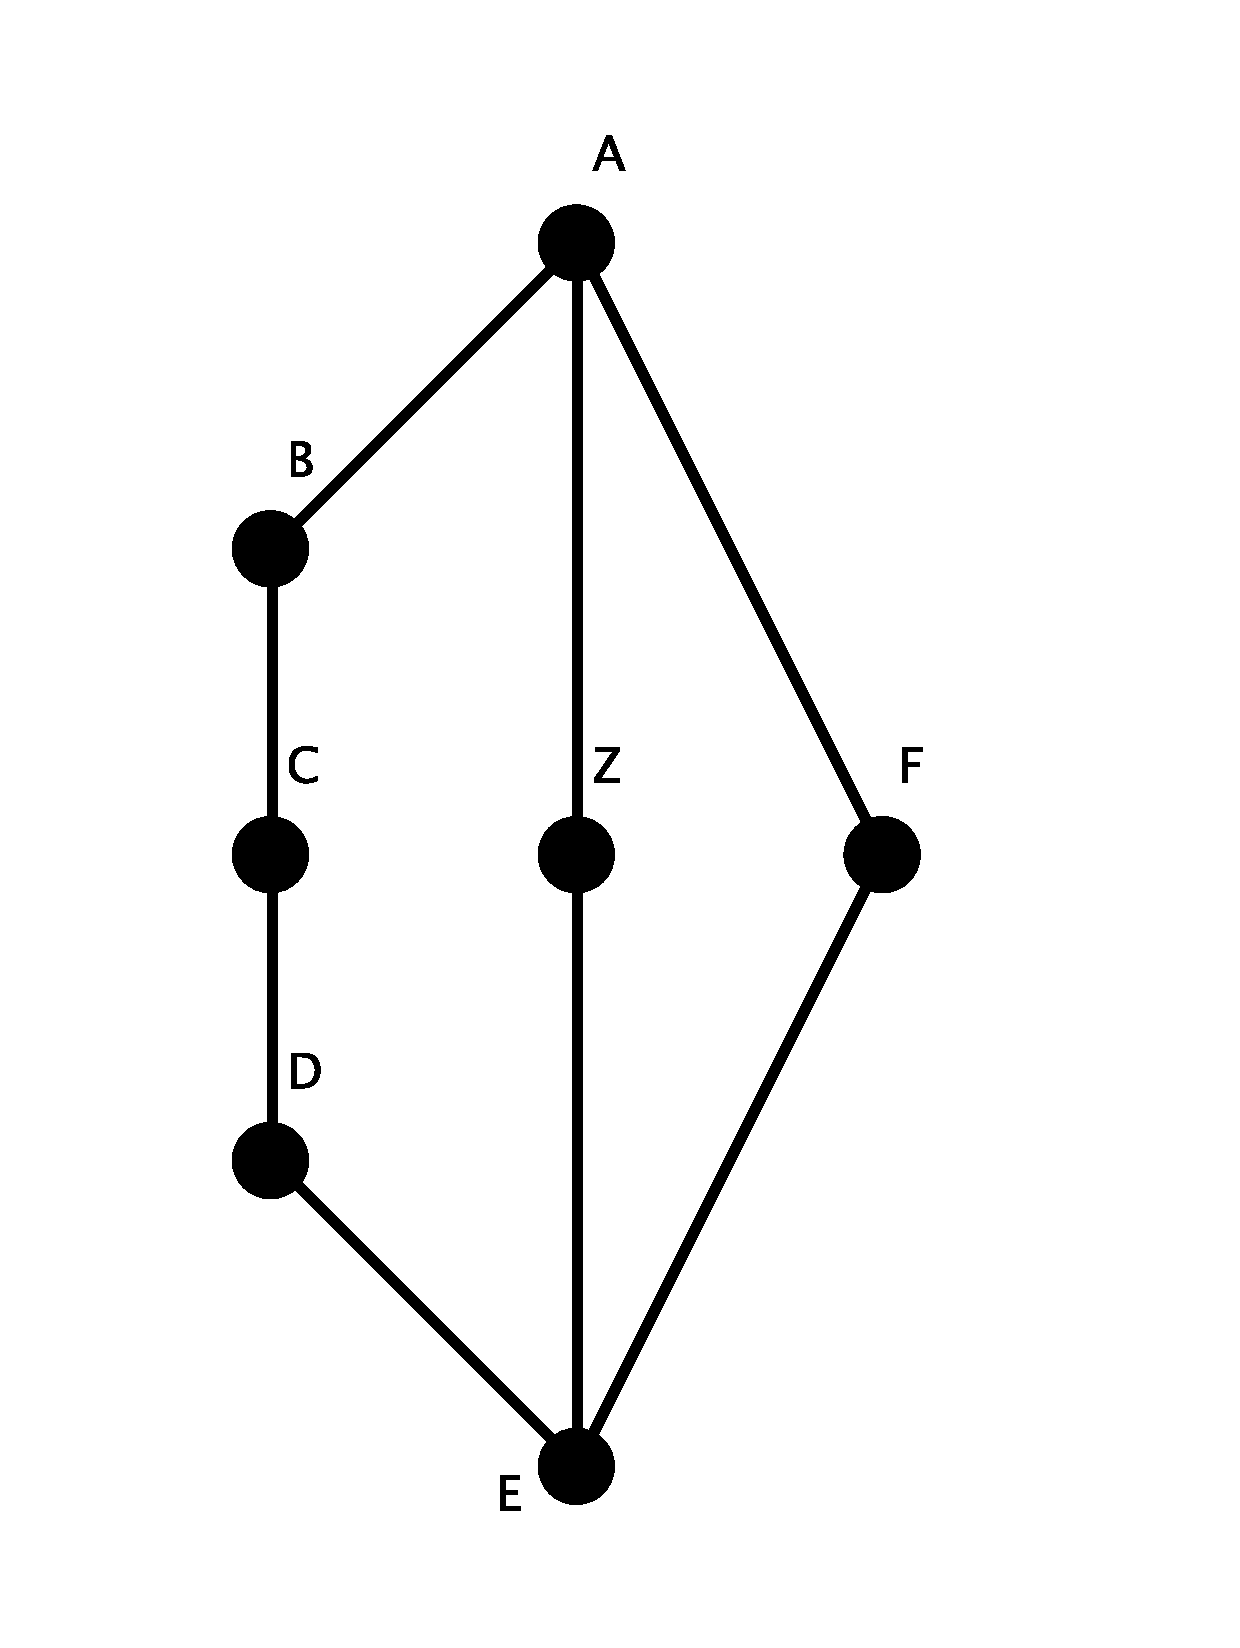
\includegraphics[width=6cm]{obrazky/siblings.pdf}
  \caption{Sourozenci konceptu $Z$}
  \label{fig.siblings}
\end{figure}

V této části popíšeme, jak vygenerovat dotazy, které jsou podobné současnému dotazu, který uživatel zadal do vyhledávače. Když jsme hledali konkrétnější dotazy, hledali jsme je v dolních sousedech; obecnější dotazy jsme hledali v~horních sousedech. Podobné dotazy budeme hledat v konceptech, které se nachází na stejné úrovni. Můžeme tak říci, že je budeme hledat v sourozencích konceptu dotazu. 

Otázkou je, jak definovat sourozence. Když se podíváme na obrázek \ref{fig.siblings}, jaké koncepty by měly být sourozenci konceptu $Z$? Když se budeme držet terminologie, která je běžná u binárních stromů, pak by sourozenci byli potomci rodiče, což by odpovídalo sourozencům $\adds{B, F}$. 

U svazů ale můžeme zvolit i opačnou cestu -- rodičové potomků. To by odpovídalo sourozencům $\adds{D, F}$. Dále můžeme říci, že sourozenci jsou všichni mezi potomky a rodiči, tj. všechny koncepty mezi konceptem $A$ a $E$, tj. $\adds{B, C, D, F}$. 

Další rozumnou možností je vzít ty koncepty, které mají stejného rodiče jako koncept $Z$ a zároveň i stejného potomka. Tomu odpovídá koncept $F$.

Pro jednu z těchto definic bychom se měli rozhodnout. Není vhodné uživateli napovídat všechny dotazy z konceptů $B, C$ a $D$, protože $D$ je konkrétnější dotaz než $C$ a $C$ je konkrétnější dotaz než $B$. Z této řady stačí uživateli navrhnout jeden dotaz. 

Pokud budeme za sourozence brát potomky rodičů, budeme mu nabízet spíše obecnější dotazy. Pokud zvolíme rodiče potomků, pak mu budeme nabízet spíše konkrétnější dotazy. 

Zvolíme tak zlatou střední cestu -- budeme mu nabízet dotazy, které jsou generovány koncepty mající společného rodiče i potomka. Zadefinujeme si funkce, které spočítají všechny horní a dolní sousedy všem prvkům množiny.

\begin{eqnarray}
\unfca(X)&=&\bigcup\adds{\upperneighbors(C)\sep C\in X}\\
\lnfca(X)&=&\bigcup\adds{\lowerneighbors(C)\sep C\in X}
\end{eqnarray}

Nyní můžeme sourozence $\sibl$ konceptu $\hledany$ zadefinovat jako
$$
\sibl_\hledany = \addh{\lnfca(\unfca(\adds{\hledany}))\cap\unfca(\lnfca(\adds{\hledany}))}\setminus\adds{\hledany}.
$$

Z této množiny už jen vytáhneme intenty a dostaneme množinu podobných dotazů
$$
Sibl=\intfca(\sibl_\hledany).
$$

Tyto dotazy setřídíme tak, že spočítáme podobnost konceptů z množiny $\sibl_\hledany$ s konceptem dotazu. Podobnost dvou konceptů spočítáme přes podobnost jejich extentů a intentů. Podobnost dvou extentů pak jednoduše definujeme jako podíl počtu společných objektů a počtu všech objektů. Podobnost dvou konceptů $\addsp{A, B}$ a $\addsp{C, D}$ je rovna
$$
\simfca(\addsp{A, B}, \addsp{C, D}) = \frac12\addk{\frac{|A\cap C|}{|A\cup C|} + \frac{|B\cap D|}{|B\cup D|}}.
$$

Návrh $s_1\in Sibl$ je relevantnější než $s_2\in Sibl$, zapíšeme $s_1\ge s_2$, právě tehdy, když pro koncepty $\addsp{A_1, B_1}, \addsp{A_2, B_2} \in \sibl_\hledany$, jejichž intenty generují $s_1$ a $s_2$, platí $\simfca(\addsp{A_1, B_1}, \hledany)\ge\simfca(\addsp{A_2, B_2}, \hledany)$. Jako první budeme zobrazovat dotaz, který je nejvíce podobný současnému dotazu $Q$.

Téma sousedních konceptů a jejich podobnosti je blíže rozebráno v článku \cite{searchsleuth} a \cite{fcasim}.


\ssection{Podobné vyhledávače}\label{ch.fcaengines}
V historii již existovaly vyhledávače, které fungovaly velice podobně jako \name. Jedná se o vyhledávače \uv{CREDO}, \uv{FooCA} a \uv{SearchSleuth}. V současné době CREDO a SearchSleuth nefungují vůbec a k použití FooCA je nutné zažádat o registraci tvůrce tohoto vyhledávače. 

\begin{description}
	\item[CREDO] Zkratka pochází z \uv{Conceptual REorganization of DOcuments}. Jeho autory jsou C. Carpineto a G. Romano. CREDO spolupracovalo s Googlem. Uživatel vložil do vyhledávače dotaz, CREDO tento dotaz nejprve poslalo pomocí SOAP API do Googlu, nechalo si vrátit prvních 100 výsledků a poté nad těmito daty provedlo FCA analýzu. CREDO počítalo pouze dolní sousedy a to do druhé úrovně. Začínalo se u největšího konceptu. Smyslem bylo, abych z těch sto výsledků, které dostal na začátku, postupně ukazoval uživateli ty odkazy, které odpovídají nějakému konceptu. 

	CREDO poté zobrazilo uživateli seznam odkazů spolu se stromovou strukturou návrhů na změnu dotazu. Tyto návrhy ale nebyly interaktivní, pouze po kliknutí na návrh se z té stovky vrácených dotazů vyfiltrovaly ty, které odpovídaly novému dotazu. Žádný nový dotaz do Google neproběhl. Detailnější informace jsou v článku \cite{credo}.

	\item[FooCA] Název vznikl ze spojení FCA a Google. Autorem je Bjoern Koester. Vyhledávač funguje na adrese \url{http://fooca.webstrategy.de}, ale vyžaduje registraci. FooCA, podobně jako CREDO, spolupracuje s webovými vyhledávači, konkrétně s Googlem a Yahoo. Uživatel vloží dotaz do Foo\-CA, ten přepošle dotaz beze změny do Google API nebo do Yahoo API a dále pracuje s navrácenými výsledky. Po skončení FCA analýzy zobrazí uživateli výsledek ve formě tabulky -- kontextu -- nebo ve formě diagramu znázorňující konceptuální svaz. 

	Detailnější informace jsou v článku \cite{fooca}.
	\item[SearchSleuth] je nejvíce podobný vyhledávači popsanému v této práci. Jeho autory jsou J. Ducrou a P. Eklund. SearchSleuth  spolupracoval s Yahoo a jeho API. Po obdržení výsledků od vyhledávače sestaví kontext, nalezne koncept dotazu a znovu vyhledá ve vyhledávači obsah intentů horních sousedů, čímž SearchSleuth získá více výsledků a může sestavit rozšířený kontext. \name{} toto provádí pomocí dodatečného OR dotazu. SearchSleuth také do kontextu nepřidává klíčová slova z dotazu. Jinak je FCA část obou vyhledávačů velice podobná. 

	Detailnější informace jsou v článku \cite{searchsleuth} a \cite{fcasim}. Podobný systém byl také použit například pro analýzu CHM souborů, proprietárního formátu Microsoftu pro nápovědu. Více informací v \cite{helpsleuth}.
\end{description} 


\newpage
\section{Výsledky vyhledávače}

\ssection{Uživatelské prostředí vyhledávače}
Současná verze vyhledávače \name{} beží na adrese \nameurl. Návod a ukázky dotazů lze nalézt na stránce \url{http://phoebe.inf.upol.cz/claseek/navod.html}. Do textového pole se vloží dotaz, který chceme položit vyhledávači, vybereme jazyk, databázi, nad kterou chceme dotaz provádět a odešleme. Výsledek vyhledávání je vidět na obrázku \ref{fig.gui.result1}

% \begin{figure}
%   \centering
%   \includegraphics[width=14cm]{obrazky/gui-zakladni.pdf}
%   \caption{Základní rozhraní vyhledávače}
%   \label{fig.gui.empty}
% \end{figure}

\begin{figure}
  \centering
  \includegraphics[width=14cm]{obrazky/gui-result1.pdf}
  \caption{Výsledek vyhledávače na dotaz \uv{fuzzy attributes}}
  \label{fig.gui.result1}
\end{figure}

% \sssection{Některé nedostatky vyhledávače}\label{ch.nedostatky}

% Podstatný požadavek je, aby se rozumné atributy nevyskytovala na všech stránkách webu. Tento problém může snadno nastat v případě, kdy jsou na všech stránkách webu stejné odkazy v navigaci. Web katedry informatiky (ale i další zkoumané weby) má na všech stránkách stejnou navigaci, takže slova, která jsou v~textech těchto odkazů, mají jen mimální šanci na to, že budou zvoleny atributem nějakého dokumentu. 

% Během výpočtu $\tfidf$ funkce hledáme taková slova, která se často vyskytují v daném dokumentu, ale co nejméně ve všech ostatních dokumentech. Funkce bohužel nezkoumá, kolikrát se dané slovo v těch ostatních dokumentech nachází, takže stačí, když se v dokumentu nachází jen jednou v navigaci a už se to bude počítat jako výskyt. 

% Kódování HTML stránky lze definovat i HTTP hlavičkou. Samotná stránka pak nemusí obsahovat element \code{<meta http-equiv='content-type'>}. Vzhledem k tomu, že \name{} HTTP hlavičky nezkoumá, použil by v tomto případě výchozí kódování \code{utf-8}. 

\ssection{Technické požadavky na HTML stránky}
Přestože \name{} podporuje další typy souborů jako PDF nebo ODT, je především stavěn pro HTML stránky. Aby vyhledávač dobře fungoval, měl by HTML dokument splňovat některá elementární pravidla. 

Vyhledávač potřebuje u každého dokumentu znát jeho název. V případě HTML stránek ho zjišťuje v elementu \code{TITLE}. Nicméně pokud ho neobsahuje nebo je jeho obsah prázdný, tak se použije poslední část URL. Obsah titulku by měl být pro každou stranu jiný. Není vhodné, aby mělo více stránek, nebo dokonce celý web, stejný titulek, protože pak je ve výsledcích vyhledávání nepůjde rozlišit jinak než jejich adresou. Toto pravidlo je důležité nejen pro tento vyhledávač, ale i pro běžné vyhledávače jako Google nebo Seznam. Zároveň se připravujeme o možnost zvýšit hodnocení stránky, pokud by klíčové slovo, které uživatel hledal, bylo v titulku. 

Další informací, kterou může z webu získat, je popisek. Ten se zapisuje do elementu \code{<META NAME='description'>}. Jeho obsahem by měl být ne příliš dlouhý text, který popisuje danou stránku. Opět by měl být unikátní pro každou stránku. Pokud stránka neobsahuje popisek, vyhledávač se pokusí ze stránky vytáhnout nějaký popisek sám, ale téměř jistě to bude horší výsledek, než ručně psaný popisek pro každou stránku zvlášť. 

HTML kód nemusí být nutně validní, ale musí dodržovat syntaxi jazyka. Nehledí se například na to, jestli element \code{IMG} obsahuje povinný atribut \code{ALT}, ale pokud nebude hodnota atributu správně ukončena uvozovkami, parser si na tom vyláme zuby. Pro převod HTML stránky do obyčejného textu se ve vyhledávači používají dvě funkce -- první používá vestavěný parser, který postupně parsuje stránku a neodpouští tak žádné chyby proti syntaxi jazyka; druhá funkce používá regulární výrazy a je tak benevolentnější, ale její výsledek je zase méně přesný. Druhá funkce se použije až v případě, kdy selže první funkce.

\ssection{Hodnocení úspěšnosti vyhledávače}
Ohodnotit, jak je \name{} úspěšný v řazení nebo v nabízených návrzích, nijak exaktně a automaticky nejde. Zbývá jen ruční zkoumání a slovní ohodnocení. 

Ve vyhledávači je uloženo několik testovacích sad dokumentů. Jedná se o weby 
\begin{itemize}
	\item \code{jakpsatweb.cz}, který se zabývá tvorbou webových stránek a podobných věcí okolo, 
	\item \code{matweb.cz}, který se zabývá především středoškolskou matematikou,
	\item \code{jakpodnikat.cz}, který se zabývá podnikáním, jak danit příjmy a podobně,
	\item \code{inf.upol.cz}, což je web katedry informatiky UP
\end{itemize}
a nakonec je ve vyhledávači použita i sada volně stažitelných odborných článků ve formátu PDF, které napsali zaměstnanci katedry informatiky UP. 

Kromě webu katedry informatiky se jedná o weby, které mají jasné zaměření každé stránky a bohatý obsah, takže na jejich webech vypadá analýza nejlépe. Web katedry informatiky je stručnější, obsahuje jisté chyby (například titulky pro každou stranu zvlášť byly vytvořeny až během psaní této práce) a obsahuje nepříjemnost v podobě opakujících se slov na každé stránce, takže jeho analýza neprobíhá nejlépe. 

\sssection{Příklady dobrých výsledků}
Analýza webu jakpodnikat.cz dává několik dobrých výsledků, pro příklad:

\begin{itemize}
	\item Na dotaz \uv{živnostenský list} vrací seznam specializací \code{+ studenti | + příjmy | + provozovna | + nemocenské | + účetnictví | + jednotný | + dědická | + odkazy | + nemovitostí | + auto}.
	\item Když k dotazu přidáme například slovo \uv{provozovna}, vyhledávač odpoví novými specializacemi \code{+ studenti | + příjmy | + zahájení | + služby | + autorský | + nemovitostí}. Zároveň přidá i podobné dotazy \code{+/- list, příjmy, živnostenský | +/- list, zahájení, živnostenský | +/- autorský, list, živnostenský | +/- nemovitostí, list, živnostenský}.
	\item Po vyhledání dotazu \uv{slevy na dani} dostaneme specializace \code{+ příjmy | + studenti | + základ | + doklady | + tisíc | + příloha | + minimální}, z nichž všechny kromě slova \uv{tisíc} dávají nějaký smysl. Seznam podobných dotazů: \code{+/- dani, příjmy | +/- dani, základ | +/- dani, doklady | +/- tisíc, dani | +/- příloha, dani}. Opět kromě dotazu, který obsahuje klíčové slovo \uv{tisíc} to má nějaký smysl. 
\end{itemize}

Dobré výsledky vrací \name{} i pro web jakpsatweb.cz: 

\begin{itemize}
	\item Pro dotaz \uv{hosting} vrátí seznam specializací \code{+ php | + serveru | + seo | + google | + weblogu | + zdarma | + nástroje | + statistiky | + domény | + anglicky}. 
	\item Pokud přidáme slovo \uv{php}, dostaneme nový seznam specializací \code{+ serveru | + knihy | + google | + zdarma | + faq | + díky | + weblogu | + xml | + seo | + statistiky} a seznam podobných dotazů: \code{+/- hosting, serveru | +/- google, hosting | +/- hosting, zdarma | +/- knihy, php | +/- php, zdarma}.
\end{itemize}

\sssection{Příklady špatných výsledků}

Ze současných databází dává většinou nejhorší výsledky web katedry informatiky. Příkladem budiž dotaz \uv{studium}, na který získáme specializace \code{+ zimní | + absolvent | + letní | + skupina | + jan | + martin | + arnošt | + činnosti | + szz | + bartl}. Většina těchto dotazů nejspíše k žádnému významnému konceptu nepovede. 

Dalším příkladem může být složitější dotaz \uv{jak vložit obrázek na stránku} nad databází jakpsatweb.cz. Vyhledávač odpoví specializacemi \code{+ obrázky | + soubor | + google | + mail}. Nabízí to dokonce slovo \uv{obrázky}, protože použitý stemmer zvolí jiný základ pro slovo \uv{obrázek} a pro \uv{obrázky}. Další návrhy nejsou o nic rozumnější. 


\ssection{API vyhledávače}

API aplikace je rozhraní, pomocí něhož může uživatel s danou aplikací komunikovat. Uživatel aplikaci posílá nějaké dotazy ve specifickém formátu a aplikace na ně opět ve specifickém formátu odpovídá. Uživatel tak může danou aplikaci používat, ačkoliv ji přímo nezkompiluje do své aplikace.  

Jak jádro vyhledávače, tak webové rozhraní poskytuje API pro uživatele. Webové API je přístupné komukoliv, konzolové API je přístupné tomu, kdo si nainstaluje vyhledávač k sobě. Webové API je RESTové, to znamená, že využívá HTTP protokol a běžné metody jako GET nebo POST. Všechna data, která vyhledávač vrací na výstupu, jsou ve formátu JSON. Pro detaily viz kapitolu \ref{ch.dokumentace}

\sssection{Získávání dat z indexu}

\name{} umožňuje získávat data o existujících indexech. Ta se získávají pomocí HTTP GET požadavku s požadovanými parametry. Je možné zjistit například informace o daném dokumentu, jaký má titulek, jakou adresu a podobně. Zároveň lze zjistit další informace o indexu, například počet všech zaindexovaných dokumentů nebo seznam URL adres všech dokumentů.

Například dotazem \code{/api.php?d=jpw\&docinfo=147\&title} zjistíme název dokumentu z databáze \code{jpw}, který má ID 147.

\sssection{Posílání vlastních dat na server}\label{ch.apipost}
API vyhledávače umožňuje poslat na server vlastní dokumenty a provést nad nimi FCA analýzu. To se děje HTTP POST požadavkem. Poslaná data musí být ve formátu JSON. \name{} tyto dokumenty přijme, zpracuje je, tj. provede úplně stejné operace, jako by budoval klasický index, vytvoří dočasný index a následně nad těmito daty provede standardní FCA analýzu, jaká byla popsána v~předchozích částech dokumentu. 

Výsledkem budou opět data ve formátu JSON, která budou obsahovat výsledek FCA analýzy. Nalezneme tam specializace, generalizace a podobné dotazy a některá další data o kontextu a konceptuálním svazu. Dále tam bude seznam dokumentů, který bude seřazený dle relevance. Výstup je prakticky stejný, jako je grafický výstup vyhledávače, pouze máme výsledky v JSON podobě. 

Tohoto můžeme využít na vylepšení výsledků běžného vyhledávače, například Googlu. Napíšeme webovou aplikaci, na které bude textové pole pro zadání dotazu. Uživatel zadá dotaz, aplikace tento dotaz přepošle API Googlu a získá výsledky pro zadaný dotaz. Následně převede výsledky z Googlu do takového formátu, kterému rozumí \name.

% Jednou z cest, kam může směřovat tento vyhledávač, je rozšíření API a napsání dalších aplikací, které toto API využívají. Jednoduchou úpravou algoritmů ve vyhledávači můžeme například vytvořit API, které bere na vstupu seznam dokumentů a na výstupu vrací kategorizovaný seznam dokumentů -- ke každému dokumentu přiřadí jednu, případně i více, kategorii. To se může hodit v případě, kdy máme velké množství dokumentů, které chceme setřídit do nějakých kategorií. Podobných způsobů využití lze jistě vymyslet více. 

\ssection{Dokumentace}\label{ch.dokumentace}
Dokumentace k jednotlivým částem programu se nachází na webu spolu se~zdrojovými kódy aplikací. K distribuci zdrojového kódu byl použit web \url{www.github.com}, přesné adresy jednotlivých projektů: Jádro vyhledávače: \url{https://github.com/havrlant/fca-search}, webové rozhraní: \url{https://github.com/havrlant/fca-search-web}.

\newpage
\section{Závěr}
Výsledkem této práce je prototyp webového vyhledávače \name{}, který primárně pracuje nad statickou sadou dokumentů. Umí prohledávat několik typů dokumentů, automaticky z dokumentů získávat název a popisek, zvládá booleovské dotazy, kontroluje překlepy a výsledné dokumenty vrací seřazené dle relevance. 

Po navrácení výsledných dokumentů provádí jejich analýzu a prostřednictvím formální konceptuální analýzy nabízí tři skupiny návrhů na úpravu dotazu: konkrétnější dotazy, obecnější dotazy a podobné dotazy. \name{} tak pomáhá uživateli upravovat dotaz tak dlouho, dokud není spokojen s výsledky vyhledávání. 

\name{} dále poskytuje veřejné webové API, díky kterému je možné vyhledávači zasílat vlastní data. Vyhledávač pak sestaví dočasný index a provede nad zaslanými daty stejnou analýzu, jako v případě statického indexu. 

Kvalita výsledků je přímo úměrná kvalitě zaindexovaných dokumentů. Pokud do~vyhledávače vložíme obsahově bohaté dokumenty, jsou návrhy většinou dobré. Celá analýza je poměrně rychlá, \name{} pro daný dotaz vrátí všechny výsledky obvykle za několik sekund. Všechny kódy jsou volně přístupné pod BSD licencí a vyhledávač tak lze případně nainstalovat na vlastní server. 

Další výzkum může proběhnout v části, která zpracovává samotné dokumenty. Například vylepšit algoritmy, které hledají atributy dokumentů, zdokonalit stemmer, zjišťovat synonyma a podobně. V části hledající návrhy je možné zavést fuzzy FCA, kdy do formálního kontextu neuložíme pouze informace o tom, zda dokument dané slovo obsahuje, ale i informaci o tom, jak moc je slovo pro dokument důležité. Je možné také rozšířit API, které \name{} nabízí a nad tímto API postavit další externí služby.

\newpage
% Diplomka používá Český styl pro BibTex, jehož autorem je David Martinek
% Zdroj: http://www.fit.vutbr.cz/~martinek/latex/czechiso.html
\bibliographystyle{czechiso}
\bibliography{citace}

\end{document}